\documentclass[14pt,ukrainian,utf8,simple]{eskdtext}

% eskdx compatibility with XeTeX
\usepackage{xecyr}

\setmainfont{STIX Two Text}
\setsansfont{Arial}

\usepackage{unicode-math}
\setmathfont{STIX Two Math}

\usepackage{polyglossia}
\setdefaultlanguage{ukrainian}

%%% Math typesetting
\usepackage{amsmath}
\usepackage{ieeetrantools}

% Units typesetting
\usepackage{siunitx}
\sisetup{output-decimal-marker = {,},
exponent-product = {\cdot}}

% Каждый раздел с новой страницы
\let\stdsection\section
\renewcommand\section{\newpage\stdsection}

% Ragged columns
\usepackage{array}
\newcolumntype{x}[1]{>{\raggedright\arraybackslash\hspace{0pt}}p{#1}}
\newcolumntype{n}[1]{>{\raggedleft\arraybackslash\hspace{0pt}}p{#1}}
% \renewcommand{\arraystretch}{1.4}

% Long tables
\usepackage{longtable}

\usepackage{subcaption}

\usepackage{enumitem}

\ESKDdepartment{Національний авіаційний університет}
\ESKDclassCode{}
\ESKDtitle{Робота транзистора з навантаженням}
%\ESKDdocName{Курсова робота}
\ESKDsignature{НАУ 17 2824000 ДД}
\ESKDauthor{Клокун~В.~Д.}
\ESKDtitleApprovedBy{Керівник роботи}{Андрєєв~В.~І.}
\ESKDchecker{Андрєєв~В.~І.}
\ESKDcolumnIX{ІКІТ СП-225}
%\ESKDtitleAgreedBy{Директор АМО ЗИЛ}{Иванов~И.~И.}
%\ESKDtitleDesignedBy{Главный инженер АМО ЗИЛ}{Петров~И.~И}

\ESKDsectAlign{section}{Center}
\ESKDsectStyle{section}{\normalsize\bfseries\MakeTextUppercase}
\ESKDsectSkip{section}{0pt}{\baselineskip}

\begin{document}
	\ESKDremoveFromStyle{formIIab}{columnII}
	\ESKDthisStyle{empty}
	
	\begin{titlepage}
	\begin{center}
			Міністерство освіти і науки України\\
			Національний авіаційний університет\\
			% Навчально-науковий інститут комп'ютерних інформаційних технологій\\
			Кафедра комп'ютерних систем та мереж

			\vspace{\fill}
			Курсова робота\\
			з дисципліни «Комп'ютерна електроніка»\\
			на тему «Робота транзистора з навантаженням»
			
			\vspace{\fill}
			
			\hspace{\fill}
			\begin{minipage}{0.5\textwidth}
			\raggedright
				Виконав:\\
				студент групи СП-225\\
				Клокун В. Д.
				
				\vspace{\baselineskip}
				
				Керівник роботи:\\
				Андрєєв В. I.
			
			\vspace{\baselineskip}
			
				Захистив: «\rule{2em}{0.4pt}» \hrulefill { }2017~р.\\
				З оцінкою \hrulefill
			\end{minipage}
			
			\vspace{2\baselineskip}
			
			Київ 2017
		\end{center}
	\end{titlepage}
	
	% \maketitle

	\newpage
	
	% Fix ESKDX retardation
	\setcounter{page}{2}
	
	\section*{Вступ}
	\addcontentsline{toc}{section}{Вступ}
	\ESKDthisStyle{formII}
		Транзистор --- напівпровідниковий елемент електронної техніки, що дозволяє керувати струмом, що протікає через нього, за допомогою зміни вхідної напруги або струму, поданих на базу, колектор або емітер. Невелика зміна вхідних величин може призводити до суттєво більшої зміни вихідної напруги та струму.
		
		Біполярний транзистор~— це напівпровідниковий прилад із~двома взаємодіючими $p$–$n$-переходами, підсилювальні властивості якого засновані на явищах інжекції та~екстракції. Умовно графічні зображення біполярних транзисторів наведені на рис.~\ref{fig:transistor-signs}. Структура~— на рис.~\ref{fig:transistors-structure}.
		
		\begin{figure}[!htbp]
		\centering
			\begin{subfigure}[t]{0.5\textwidth - 0.5em}
			\centering
				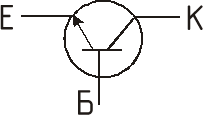
\includegraphics[height = 2.5\baselineskip]{assets/npn-transistor-sign.png}
			\caption{}
			\label{subfig:npn-transistor}
			\end{subfigure}%
			\quad
			\begin{subfigure}[t]{0.5\textwidth - 0.5em}
			\centering
				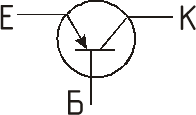
\includegraphics[height = 2.5\baselineskip]{assets/pnp-transistor-sign.png}
			\caption{}
			\label{subfig:pnp-transistor}
			\end{subfigure}
		\caption{Умовно-графічні зображення біполярних транзисторів: \subref{subfig:npn-transistor}~—~\mbox{$n$–$p$–$n$}-типу, \subref{subfig:pnp-transistor}~—~\mbox{$p$–$n$–$p$}-типу}
		\label{fig:transistor-signs}
		\end{figure}
		
		\begin{figure}[!htbp]
		\centering
			\begin{subfigure}[t]{0.5\textwidth - 0.5em}
			\centering
				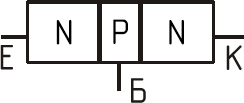
\includegraphics[height = 2\baselineskip]{assets/npn-transistor-cross-section.png}
			\caption{}
			\label{subfig:npn-transistor-cross-section}
			\end{subfigure}%
			\quad
			\begin{subfigure}[t]{0.5\textwidth - 0.5em}
			\centering
				
\includegraphics[height = 2\baselineskip]{assets/pnp-transistor-cross-section.png}
			\caption{}
			\label{subfig:pnp-transistor-cross-section}
			\end{subfigure}
		\caption{Структура біполярних транзисторів: \subref{subfig:npn-transistor}~—~\mbox{$n$–$p$–$n$}-типу, \subref{subfig:pnp-transistor}~—~\mbox{$p$–$n$–$p$}-типу}
		\label{fig:transistors-structure}
		\end{figure}
		
		% Дана курсова робота виконується з~метою закріплення та~поглиблення теоретичних знань та~навичок в~області біполярних транзисторів. Транзистори є основними елементами сучасної електроніки. Тому під час виконання курсової роботи слід побудувати пряму навантаження на~вольт-амперній характеристиці для заданого типу транзистора та~режиму; вибрати робочу точку та визначити графоаналітичним методом $h$-параметри, коефіцієнти підсилення та~значення зворотного струму колектора $I_{\text{КЗ}}$ для заданої температури.
		
		Завдання на дану курсову роботу наведене у табл.~\ref{tab:coursework-task}.
		\begin{table}[!htbp]
		\centering
			\begin{tabular}{|c|c|c|c|c|}
				\hline
					Варіант & Транзистор & $E_{\text{К}},~\si{\volt}$ & $R_{\text{К}},~\si{\ohm}$ & $t, \si{\degreeCelsius}$\\
				\hline
					28      & КТ104      & $20$                      & $1000$                    & $120$\\
				\hline
			\end{tabular}
		\caption{Завдання на курсову роботу}
		\label{tab:coursework-task}
		\end{table}
	
	\section*{Довідкові дані транзистора}
	\addcontentsline{toc}{section}{Довідкові дані транзистора}
		КТ104В, КТ104Б, КТ104В, КТ104Г~— це кремнієві біполярні планарно-епітаксіальні \mbox{$p$–$n$–$p$}-транзистори, призначені для роботи в схемах радіоприймачів та іншій апаратурі. Корпус металевий, герметичний, з гнучкими виводами. Маса транзистора не більше \SI{0,5}{\gram}.
		
		\begin{figure}[!htbp]
		\centering
			\begin{subfigure}[b]{0.3\textwidth}
			\centering
				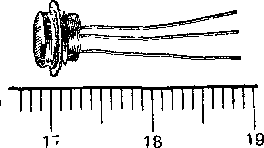
\includegraphics[height = 3\baselineskip]{assets/01-kt104-view.png}
			\caption{}
			\label{subfig:kt104-view}
			\end{subfigure}
			\quad
			\begin{subfigure}[b]{0.3\textwidth}
			\centering
				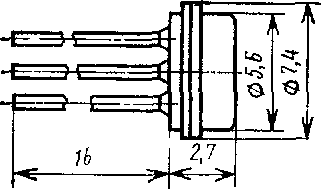
\includegraphics[height = 3\baselineskip]{assets/02a-kt104-view-sizes.png}
			\caption{}
			\label{subfig:kt104-sizes}
			\end{subfigure}
			\quad
			\begin{subfigure}[b]{0.3\textwidth}
			\centering
				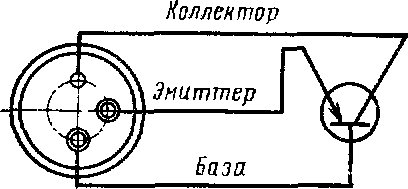
\includegraphics[height = 3\baselineskip]{assets/02b-kt104-view-disambig.png}
			\caption{}
			\label{subfig:kt104-disambig}
			\end{subfigure}
		\caption{Транзистор КТ104: \subref{subfig:kt104-view}~— зовнішній вигляд, \subref{subfig:kt104-sizes}~— габарити, \subref{subfig:kt104-disambig}~— цоколь}
		\end{figure}
		
		Електричні параметри транзистора КТ104В наведені у таблиці \ref{tab:ktelectricparams}.
		\begin{longtable}[c]{|x{0.22\textwidth}|c|r|r|r|r|r|r|r|}
			\hline
				Найменування                                      & Позн.              & \multicolumn{2}{c|}{Значення} & \multicolumn{5}{c|}{Режим виміру} \\
				\cline{3-4} \cline{5-9}
				& & Мін. & Макс. & $U_{\text{К}}, \si{\volt}$ & $U_{\text{Е}}, \si{\volt}$ & $I_{\text{К}}, \si{\milli\ampere}$ & $I_{\text{Б}}, \si{\milli\ampere}$ & $I_{\text{Е}}, \si{\milli\ampere}$ \\
			\hline
			\endhead
			\caption{Електричні параметри транзистора КТ104В}
			\label{tab:ktelectricparams}
			\endfoot
			
				Зворотний~струм колектора, \si{\micro\ampere}                                                                  & $I_{\text{КБЗ}}$   &     &  1    & 15    &       &    &   & \\
				при $T_{\text{С}} = \SI{+100}{\celsius}$                                                                       &                    &     & 15    & 10    &       &    &   & \\
				при $T_{\text{С}} = \SI{-060}{\celsius}$                                                                       &                    &     &  1    & 15    &       &    &   & \\
				\hline
				Зворотний~струм емітера, \si{\micro\ampere}                                                                    & $I_{\text{ЕБЗ}}$   &     & 1     &       & 10    &    &   & \\
				при $T_{\text{С}} = \SI{+100}{\celsius}$                                                                       &                    &     & 10    &       & 5     &    &   & \\
				при $T_{\text{С}} = \SI{-060}{\celsius}$                                                                       &                    &     & 1     &       & 10    &    &   & \\
				\hline
				Гранична напруга транзистора ($T_{\text{С}} = -60 \ldots +100~\si{\celsius}$), \si{\volt}                      & $U_{\text{КЕЗгр}}$ & 15  &       &       &       &    &   & 10\\
				\hline
				Напруга насичення колектор~--- емітер, \si{\volt}                                                              & $U_{\text{КЕнас}}$ &     & 0{,}5 &       &       & 10 & 1 & \\
				\hline
				Напруга насичення база~--- емітер, \si{\volt}                                                                  & $U_{\text{БЕнас}}$ &     & 1     &       &       & 10 & 1 & \\
				\hline
				Вхідний опір транзистора в режимі малого сигналу, \si{\ohm}                                                    & $h_{11\text{б}}$   & 120 &       & 15    &       &    &   & 1 \\
				\hline
				Коефіцієнт передачі струму в режимі малого сигналу у схемі з ЗЕ                                                & $h_{21\text{е}}$   & 40  & 160   & 5     &       &    &   & 1 \\
				при $T_{\text{С}} = \SI{+100}{\celsius}$                                                                       &                    & 30  & 380   & 5     &       &    &   & 1 \\
				при $T_{\text{С}} = \SI{-060}{\celsius}$                                                                       &                    & 25  & 160   & 5     &       &    &   & 1 \\
				\hline
				Гранична частота коефіцієнта передачі струму, \si{\mega\hertz}                                                 & $fh_{21\text{б}}$  & 5   &       & 5     &       &    &   & 1 \\
				\hline
				Ємність колекторного переходу (при $f = \SI{465}{\kilo\hertz}$), \si{\pico\farad}                              & $C_{\text{К}}$     &     & 50    & 5     &       &    &   &\\
				\hline
				Ємність емітерного переходу (при $f = \SI{465}{\kilo\hertz}$), \si{\pico\farad}                                & $C_{\text{Е}}$     &     & 10    &       & 0{,}5 &    &   &\\
				\hline
				Стала часу ланцюгу зворотного зв'язку на високій частоті (при $f = \SI{3}{\mega\hertz}$), \si{\nano\second}    & $\tau_{\text{К}}$  &     & 3     & 5     &       &    &   & 1\\
			\hline
		\end{longtable}
			
		Максимально допустимі параметри для транзистора КТ104В наведені у таблиці \ref{tab:ktmaxparams}.
		
		\begin{longtable}[c]{|x{0.5\textwidth}|c|r|}
			\hline
				Найменування & Позначення & Значення \\
			\hline
			\endhead
			\caption{Максимально допустимі параметри для транзистора КТ104В}
			\label{tab:ktmaxparams}
			\endfoot
			
				Постійний струм колектора, \si{\milli\ampere} & $I_{\text{К max}}$ & 50 \\
				\hline
				Постійна напруга колектор~— база, \si{\volt}        & $U_{\text{КБ max}}$ & 15 \\
				\hline
				Постійна напруга колектор~— емітер (при запираючій напрузі $U_{\text{ЕБ}} = \SI{0,5}{\volt}$ або при $R_{\text{Б}} \leqslant \SI{10}{\kilo\ohm}$), \si{\volt} & $U_{\text{КЕ max}}$ & 15 \\
				\hline
				Постійна напруга емітер~— база, \si{\volt} & $U_{\text{ЕБ max}}$ & 10 \\
				\hline
				Постійна розсіювана потужність колектора, \si{\milli\watt} & $P_{\text{К max}}$ & 150 \\
				\hline
				Тепловий опір перехід~— середовище, \si[per-mode = symbol, bracket-unit-denominator = false]{\celsius\per\milli\watt} & $R_{\text{т, п—с}}$ & 0{,}4 \\
				\hline
				Допустима температура навколишнього середовища, \si{\celsius} & & $\num{-60} \ldots \num{+100}$ \\
			\hline
		\end{longtable}
			
	\section*{Вольт-амперні характеристики транзистора}
	\addcontentsline{toc}{section}{Вольт-амперні характеристики транзистора}
		Біполярні транзистори мають чотири статичні вольт-амперні характеристики (ВАХ):
		\begin{enumerate}[label=\arabic*.]
			\item Вхідні~— зв'язують струм і напругу на вході транзистора.
			\item Вихідні~— зв'язують струм і напругу на виході транзистора.
			\item Характеристики передачі~— зв'язують струми чи напруги на виході транзистора зі струмами чи напругами на вході.
			\item Характеристики зворотного зв'язку~— зв'язують напруги чи струми на вході зі струмами чи напругами на виході.
		\end{enumerate}
		
		Розглянемо для прикладу вхідні та вихідні ВАХ.
		
		\begin{figure}[!htbp]
		\centering
			\begin{subfigure}[t]{0.5\textwidth - 0.5em}
			\centering
				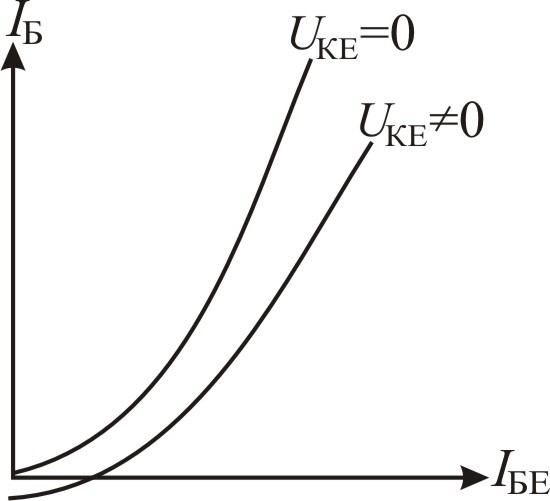
\includegraphics[height = 6\baselineskip]{assets/vac-input.jpg}
			\caption{}
			\label{subfig:vac-input}
			\end{subfigure}
			~
			\begin{subfigure}[t]{0.5\textwidth - 0.5em}
			\centering
				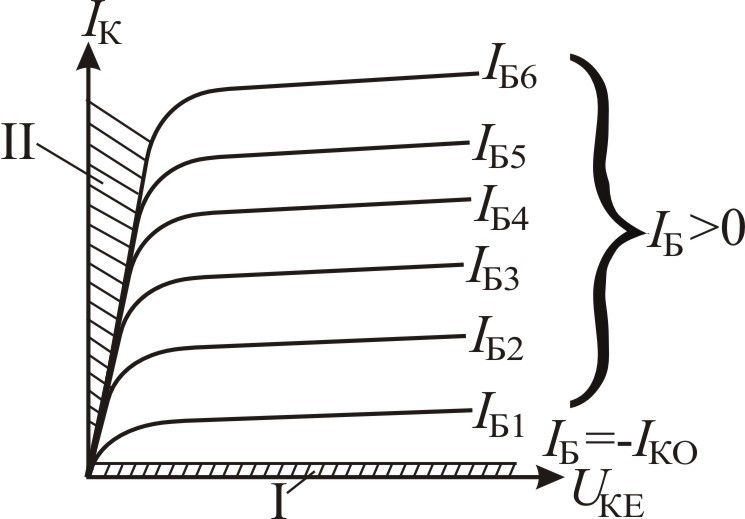
\includegraphics[height = 6\baselineskip]{assets/vac-output.jpg}
			\caption{}
			\label{subfig:vac-output}
			\end{subfigure}
		\caption{Статичні вольт-амперні характеристики транзистора, ввімкненого за~схемою з~загальним емітером: \subref{subfig:vac-input}~— вхідні характеристики, \subref{subfig:vac-output}~— вихідні характеристики}
		\label{fig:generic-vac}
		\end{figure}
		
		Видно, що при напрузі $U_{\text{КЕ}} = 0$ вхідна характеристика починається на початку координат (рис.~\ref{subfig:vac-input}). При збільшенні $U_{\text{КЕ}}$ ($U_{\text{КЕ}} \neq 0$) вхідна характеристика зміщується вправо і вниз. Для схеми з загальним емітером вхідні характеристики описуються функціональною залежністю~\eqref{eqn:input-characteristics}.
		\begin{equation}
		\label{eqn:input-characteristics}
			U_{\text{БЕ}} = f\left( I_{\text{Б}} \right), \quad \text{при}~U_{\text{КБ}} = \text{const}.
		\end{equation}
		
		Вихідні характеристики (рис.~\ref{subfig:vac-output}) дозволяють визначити режими роботи транзистора: область~I відповідає режиму відсічення, область~II~— режиму насичення, область~III — активному режиму. Вихідні характеристики визначаються функціональною залежністю~\eqref{eqn:output-characteristics}.
		\begin{equation}
		\label{eqn:output-characteristics}
			I_{\text{К}} = f\left( U_{\text{КБ}} \right), \quad \text{при}~I_{\text{Б}} = \text{const}.
		\end{equation}
		
		Вольт-амперні характеристики транзистора, вказаного у завданні на курсову роботу, наведені на рис.~\ref{fig:kt104-vac}. Згідно з інформацією, наведеною у довіднику, $\Delta I_{\text{Б}} = \SI{0,2}{\milli\ampere}$.
		
		\begin{figure}[!htbp]
		\centering
			\begin{subfigure}[t]{0.5\textwidth - 0.5em}
			\centering
				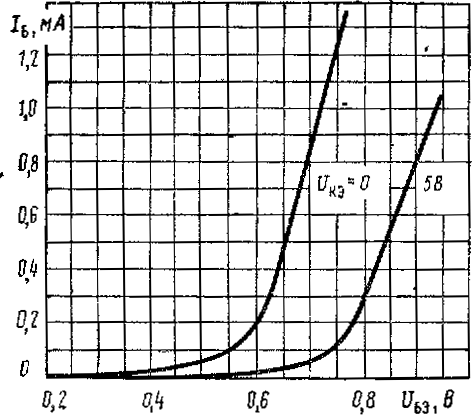
\includegraphics[height = 9\baselineskip]{assets/03-kt104-vac-input.png}
			\caption{}
			\label{subfig:kt104-vac-input}
			\end{subfigure}%
			\quad
			\begin{subfigure}[t]{0.5\textwidth - 0.5em}
			\centering
				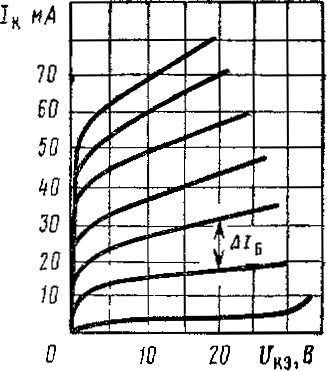
\includegraphics[height = 9\baselineskip]{assets/03-kt104-vac-output.png}
			\caption{}
			\label{subfig:kt104-vac-output}
			\end{subfigure}
		\caption{Вольт-амперні характеристики транзистора КТ104В: \subref{subfig:kt104-vac-input}~—~вхідні~характеристики, \subref{subfig:kt104-vac-output}~— вихідні~характеристики}
		\label{fig:kt104-vac}
		\end{figure}
	
	\section*{Побудова прямої навантаження}
	\addcontentsline{toc}{section}{Побудова прямої навантаження}
		Відомо, що під час роботи біполярного транзистора з навантаженням зміни струму колектора будуть залежати від змін струму~$I_{\text{Б}}$ і~напруги~$U_{\text{КЕ}}$. Такий принцип роботи транзистора іноді називають динамічним, а характеристики~— динамічними.
		
		Звернувши увагу на вольт-амперні характеристики~(рис.~\ref{fig:generic-vac}), спостерігається залежність:
		\begin{equation}
		\label{eqn:u-ke}
			U_{\text{КЕ}} = E_{\text{К}} - I_{\text{К}} R_{\text{К}}.
		\end{equation}
		
		Залежність~\eqref{eqn:u-ke} можна привести до такої форми:
		\begin{equation}
		\label{eqn:ik}
			I_{\textnormal{К}} = \frac{E_\textnormal{K} - U_{\textnormal{КЕ}}}{R_\textnormal{K}} = \frac{E_{\textnormal{K}}}{R_{\textnormal{K}}} - \frac{U_{\textnormal{КЕ}}}{R_{\textnormal{K}}},
		\end{equation}
		де $I_{\textnormal{К}}$ --- вихідний струм, $E_{\textnormal{К}}$ --- електрорушійна сила джерела живлення, $U_{\textnormal{КЕ}}$ --- напруга «колектор-емітер», $R_{\textnormal{К}}$ --- опір резистора навантаження.
		
		Пряма, що описується рівнянням~\eqref{eqn:ik}, називається \emph{навантажувальною}. Навантажувальна пряма — це пряма, що однозначно пов'язує струм і~напругу на виході, та є траєкторією руху робочої точки в посилюючому режимі роботи біполярного транзистора, тобто при включенні в ланцюг навантажувального резистора $R_{\textnormal{К}}$.
		
		Для побудови навантажувальної прямої на сімействі вихідних характеристик достатньо двох точок. Оскільки з формули~\eqref{eqn:ik} видно, що при $I_{\textnormal{К}} = 0$, $U_{\textnormal{КЕ}} = E_{\textnormal{К}}$, то для знаходження першої точки навантажувальної прямої --- точки $K$ --- необхідно відкласти на осі абсцис величину $E_{\textnormal{К}}$. У цій точці транзистор замкнений. Для знаходження другої точки навантажувальної прямої --- точки $B$ --- використаємо величину $U_{\textnormal{КЕ}}$ таким чином: припустимо, що $U_{\textnormal{КЕ}} = 0$, тоді $I_{\textnormal{К}} = \frac{E_{\textnormal{К}}}{R_{\textnormal{К}}}$. Пряма $BK$ і буде шуканою навантажувальною прямою.
		
		Виконаємо розрахунки відповідно до отриманого завдання. Для цього знайдемо абсцису точки~$K$:
		\[
			x_K = E_{\text{К}} = \SI{20}{\volt}.
		\]
		Далі знаходимо ординату точки~$B$:
		\[
			y_B = \frac{E_{\text{К}}}{R_{\text{К}}}
			    = \frac{\SI{20}{\volt}}{\SI{1000}{\ohm}}
			    = \SI{0,02}{\ampere}
			    = \SI{20}{\milli\ampere}.
		\]
		
		Таким чином, отримали дві точки: $K(\SI{20}{\volt}; \SI{0}{\milli\ampere})$ і~$B(\SI{0}{\volt}; \SI{20}{\milli\ampere})$. За координатами отриманих точок на сімействі вихідних характеристик будуємо навантажувальну пряму~(рис.~\ref{fig:kt104-vac-output-loadline}).
		
		\begin{figure}[!htbp]
		\centering
			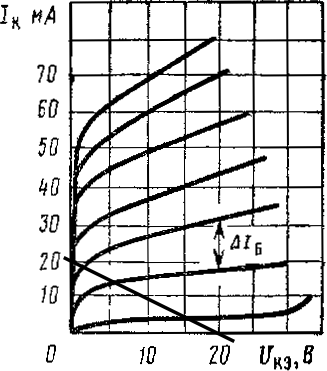
\includegraphics[height = 9\baselineskip]{assets/04-kt104-output-loadline.png}
		\caption{Сімейство вихідних вольт-амперних характеристик транзистора~КТ104В з навантажувальною прямою}
		\label{fig:kt104-vac-output-loadline}
		\end{figure}

	\section*{Графічне визначення $K_U$, $K_I$, $K_P$}
	\addcontentsline{toc}{section}{Графічне визначення $K_U$, $K_I$, $K_P$}
		За допомогою амплітудних значень, що були визначені графічно~(рис.~7), визначаємо коефіцієнти посилення. Спочатку запишемо їх.
		
		\begin{longtable}[c]{|x{0.3\textwidth}|c|r|}
			\hline
				Параметр & Позначення & Значення\\
			\hline
			\endhead
			\hline
			\caption{Амплітудні значення, визначені графічно}
			\label{tab:amplitude-param}
			\endfoot
			
				Амплітудне значення вихідного~струму & $I_{\text{КМ}}$ & $\SI{8}{\milli\ampere} = \SI{0,008}{\ampere}$\\
				\hline
				Амплітудне значення вхідного~струму  & $I_{\text{БМ}}$ & $\SI{0,2}{\milli\ampere} = \SI{0,0002}{\ampere}$\\
				\hline
				Амплітудне значення вихідної~напруги & $U_{\text{КМ}}$ & \SI{7}{\volt}\\
				\hline
				Амплітудне значення вхідної~напруги  & $U_{\text{БМ}}$ & \SI{0,03}{\volt}\\
				\hline
		\end{longtable}
		
		Визначимо коефіцієнт підсилення по напрузі~$K_I$:
		\[
			K_I = \frac{I_{\text{ВИХ}}}{I_{\text{ВХ}}}
			    = \frac{I_{\text{КМ}}}{I_{\text{БМ}}}
				= \frac{\SI{8}{\milli\ampere}}{\SI{0,2}{\milli\ampere}}
				= \num{40}.
		\]
		
		Далі визначимо коефіцієнт підсилення по струму~$K_U$:
		\[
			K_U = \frac{U_{\text{КМ}}}{U_\text{БМ}}
			    = \frac{\SI{7}{\volt}}{\SI{0,03}{\volt}}
				= \num{233,3}.
		\]
		
		Визначимо коефіцієнт підсилення по потужності~$K_P$:
		\begin{IEEEeqnarray*}{rCcCcCcCcl}
			K_P &=& \frac{P_{\text{ВИХ}}}{P_{\text{ВХ}}}
			    &=& \frac{I_{\text{ВИХ}} \cdot U_{\text{ВИХ}}}{I_{\text{ВХ}} \cdot U_{\text{ВХ}}}
			    &=& K_I \cdot K_U\\[2\jot]
			    & &	&=& \frac{\SI{0,008}{\ampere} \cdot \SI{7}{\volt}}
				       {\SI{0,0002}{\ampere} \cdot \SI{0,03}{\volt}}
				&=& \num{40} \cdot \num{233,3}
			    &=& \num{9333,3}.
		\end{IEEEeqnarray*}
	
	\section*{Визначення параметрів $h_{11}$, $h_{12}$, $h_{21}$, $h_{22}$}
	\addcontentsline{toc}{section}{Визначення параметрів $h_{11}$, $h_{12}$, $h_{21}$, $h_{22}$}
		Величини, що зв'язують малі збільшення струмів і напруг називаються диференціальними параметрами транзисторів. Для транзисторів запропоновано багато систем параметрів, однак, основними вважаються змішані (\emph{hybrid}) параметри, які позначають літерою $h$.
		
		У системі $h$-параметрів за незалежні змінні обирають вхідний струм $I_1$ і напругу $U_2$, а за залежні --- вхідну напругу $U_1$ і вихідний струм $I_2$. Це пов'язано з малим вхідним і великим вихідним опорами транзистора. Для схеми ввімкнення із загальним емітером це такі величини:
			\begin{itemize}
				\item вхідний струм $I_{\text{Б}}$ і напруга $U_{\text{БЕ}}$.
				\item вихідний струм $I_{\text{К}}$ і напруга $U_{\text{КЕ}}$.
			\end{itemize}
			
		Тоді система рівнянь, що пов'язує $h$-параметри має такий вигляд:
		\begin{equation}
			\begin{cases}
				U_{\text{БЕ}} = h_{11} I_{\text{Б}} + h_{12} U_{\text{КЕ}}\\
				I_{\text{К}} = h_{21} I_{\text{Б}} + h_{22} U_{\text{КЕ}}\\
			\end{cases}
			\label{eq:hparamsys}
		\end{equation}
		
		Із системи рівнянь \eqref{eq:hparamsys} випливає фізичний зміст і назви $h$-па\-ра\-мет\-рів. Вхідний опір транзистора при короткому замиканні на виході для змінної складової струму:
			\[
				h_{11} = \frac{U_1}{I_1}, \, U_2 = 0.
			\]
		
		Коефіцієнт зворотного зв'язку за напругою при розімкнутому вході для змінної складової струму:
			\[
				h_{12} = \frac{U_1}{U_2}, \, I_1 = 0.
			\]
			
		Диференціальний коефіцієнт передачі струму:
			\[
				h_{21} = \frac{I_2}{I_1}, \, U_2 = 0.
			\]
			
		Вихідна провідність транзистора при розімкнутому вході для змінної складової струму:
			\[
				h_{22} = \frac{I_2}{U_2}, \, I_1 = 0.
			\]
			
		Для визначення $h$-параметрів також можна використовувати графо\-ан\-а\-лі\-тич\-ний спосіб. Варто зазначити, що він має невисоку точність.
		
		Для визначення $h$-параметрів графоаналітичним способом на вхідних і~вихідних характеристиках навколо робочої точки необхідно побудувати трикутники. На сімействі вхідних характеристик у робочій точці~$A$ будують трикутник~$ABC$. З~точки~$A$ проводять прямі, рівнобіжні осі абсцис і~осі ординат до перетинання з~другою характеристикою в~точках~$B$ і~$C$. З~отриманого характеристичного трикутника знаходять всі необхідні величини для обчислення~$h_{\text{11Е}}$, $h_{\text{12Е}}$. Відрізок~$AB$ є $\Delta U_{\text{БЕ}}$, а $AC$~— збільшення $\Delta I_{\text{Б}}$.
		
		Збільшення напруги колектора визначається як різниця напруг, при яких знімалися характеристики:
		\[
			\Delta U_{\text{КЕ}} = U''_{\text{КЕ}} - U'_{\text{КЕ}}
			                     = \SI{5}{\volt} - \SI{0}{\volt}
								 = \SI{5}{\volt}.
		\]
		
		Тоді:
		\[
			h_{\text{11Е}} = \frac{\Delta U_{\text{БЕ}}}{\Delta I_{\text{Б}}}
			               = \frac{AB}{AC}
						   = \frac{\SI{0,18}{\volt}}{\SI{1,2}{\milli\ampere}}
						   = \frac{\SI{0,18}{\volt}}{\SI{0,0012}{\ampere}}
						   = \SI{150}{\ohm},
		\]
		\[
			h_{\text{12Е}} = \frac{\Delta U_{\text{БЕ}}}{\Delta U_{\text{КЕ}}}
			               = \frac{AB}{U''_{\text{КЕ}} - U'_{\text{КЕ}}}
						   = \frac{\SI{0,18}{\volt}}{\SI{5}{\volt}}
						   = \num{0,036}.
		\]
		
		У робочій точці $A'$ за вихідними характеристиками можна визначити параметри $h_{\text{21Е}}$ і $h_{\text{22Е}}$. Проводячи з точки $A'$ вертикальну пряму до перетинання з наступною характеристикою (точка $D'$), знаходимо збільшення струму колектора $\Delta I_{\text{К}}$ при $U'_{\text{КЕ}} = \mathrm{const}$. Відрізок $A'D'$ показує на збільшення струму бази $\Delta I_{\text{Б}} = I_{\text{Б5}} - I_{\text{Б4}}$.
		
		Тоді:
		\[
			h_{\text{21Е}} = \frac{\Delta I_{\text{К}}}{\Delta I_{\text{Б}}}
			               = \frac{A'D'}{I_{\text{Б5}} - I_{\text{Б4}}}
						   = \frac{\SI{8}{\milli\ampere}}{\SI{1,2}{\milli\ampere}}
						   = \frac{\SI{0,008}{\ampere}}{\SI{0,0012}{\ampere}}
						   = \num{6,6667}.
		\]
		
		Для визначення параметра $h_{\text{22Е}}$ з точки $A'$ проводять пряму, рівнобіжну осі абсцис, необхідної довжини для виміру збільшення струму $\Delta I'_{\text{К}} = B'C'$. За точками визначимо збільшення напруги колектора $\Delta U'_{\text{БЕ}}$. Тоді:
		\[
			h_{\text{22Е}} = \frac{\Delta I'_{\text{К}}}{\Delta U'_{\text{БЕ}}}
			               = \frac{B'C'}{A'B'}
						   = \frac{\SI{7}{\milli\ampere}}{\SI{24}{\volt}}
						   = \frac{\SI{0,007}{\ampere}}{\SI{24}{\volt}}
						   = \SI{0,000292}{\siemens}.
		\]
		
	\section*{Визначення $I_{\textnormal{КЗ}}$ при заданій температурі}
	\addcontentsline{toc}{section}{Визначення $I_{\textnormal{КЗ}}$ при заданій температурі}
		Зворотний струм колектора~$I_{\text{КЗ}}$ залежить від температури~$t$. Зі збільшенням температури на~\SI{10}{\degreeCelsius} струм збільшується в 2~рази.
		
		Довідковий матеріал вказує, що при температурі $t = \SI{100}{\degreeCelsius}$ максимальний струм~$I_{\text{КЗ}} = \SI{15}{\micro\ampere}$. Використовуючи вищезгадане правило, проведемо обчислення~(табл.~\ref{tab:i-kz-computation}).
		\begin{longtable}[c]{|l|r|}
			\hline
				$t$, \si{\degreeCelsius} & $I_{\text{КЗ}}$, \si{\micro\ampere}\\
			\hline
			\endhead
			\hline
			\caption{Покрокове обчислення зворотного струму~$I_{\text{КЗ}}$ для заданого значення температури~$t$}
			\label{tab:i-kz-computation}
			\endfoot
			
			100 & 15\\
			\hline
			110 & $15 \cdot 2 = 30$\\
			\hline
			120 & $30 \cdot 2 = 60$\\
		\end{longtable}
		
	\section*{Література}
	\addcontentsline{toc}{section}{Література}
		\begin{enumerate}[label=\arabic*.]
			\item \textit{Андрєєв В.~І, Андрєєв О.~В.} Комп'ютерна електроніка: навчальний посібник. —~К.: НАУ, 2009. —~320~с.
			\item \textit{Андрєєв В.~І., Андрєєв О.~В.} Комп'ютерна електроніка: лабораторний практикум. —~К.: НАУ, 2013. —~84~с.
			\item \textit{Брежнєва К.М., Гантман Є.І., Давидова Т.М. та ін.} Під редакцією Перельмана Б.Л. Транзистори для апаратури широкого застосування: довідник. —~М.: Радіо та зв’язок, 1981р. —~656 с.
			\item \textit{Андрєєв В.І., Андреєв О.В.} Комп’ютерна електроніка. К.: видавництво ДУІКТ, 2010. —~320 с.
		\end{enumerate}
		
	\newpage
	
	\renewcommand{\ESKDtheColumnII}{НАУ 16 2824000 ПЗ}
	
	\ESKDthisStyle{formII}
	\tableofcontents
	
\end{document}